\documentclass[50pt]{article}
\usepackage[utf8]{inputenc}
\usepackage[spanish]{babel}
\usepackage[margin=2.5cm]{geometry}
\usepackage{amsmath,amssymb}
\usepackage{graphicx}
\usepackage{float}
\usepackage{enumitem}

\title{
    \vspace{-2.5cm} 
    {\centering 
\includegraphics[width=1.0\textwidth]{banner.png} \\[1cm]}
    \textbf{Funciones escalares de varias variables} \\[1cm]
    \large E.D. 1.1. Ejercicios \\[4cm]
}  

\author{
    253110213 - Flores Soria Ximena \\
    253110111 - Martinez Castillo Dair \\
    253110169 - Garduño Reyes Alejandro \\
    253110012 - Alvarado Villegas Gael Salvador \\
    253110534 - Belmontes Flores Joshua Shadai \\[4cm]
}

\date{Septiembre, 2026}

\begin{document}
\maketitle
\begin{center}
    \vspace{1cm}
    
    \textbf{GRUPO:} TID-401 \\[0.8cm]
    
    \textbf{Docente:} Rubén Ramírez Gómez

\end{center}


\newpage

\section*{Ejercicio 1: Optimización de costos en servidores "Serverless"}
\noindent\textbf{Funci\'on:} $C(n,t) = 0.000016 \cdot n \cdot t$\\
 
\subsection*{1. Variables independientes y dependiente}
\begin{itemize}[leftmargin=1.5em]
\item \textbf{Independientes:} n -- (número de ejecuciones en millones), t -- (tiempo promedio de ejecución por proceso en segundos)
\item \textbf{Dependiente:} C -- (costo mensual en dólares)
\end{itemize}
El equipo puede elegir o proyectar n y t, mientras que el costo C se calcula a partir de ellas, por eso depende de ambas.
\subsection*{2. Dominio}
\{(n,t) : n $\geq$ 0, 0.1 $\leq$ t $\leq$ 900\} \\
\subsection*{3. Rango}
[0, $\infty$).\\\\
Valor mínimo: Para $n = 0$ y cualquier $t$, $C(0, t) = 0$.Para $n > 0$, el costo mínimo para un $n$ dado se alcanza con $t = 0.1$: $C(n, 0.1) = 0.0000016 \times n$.Por ende, el costo no puede ser negativ
\subsection*{4. Representaci\'on tabular}
Los datos de la tabla original corresponden a la constante 0.016 (por ejemplo, $0.016 \cdot 10 \cdot 1 = 0.16$), por lo que las celdas faltantes se calculan con $C = 0.016 \cdot n \cdot t$:
\begin{align*}
C(100,5) &= 0.000016(100)(5) = 0.008\\
C(500,1) &= 0.000016(500)(1) = 0.008\\
C(500,10) &= 0.000016(500)(10) = 0.08
\end{align*}
\begin{center}
\begin{tabular}{|c|c|c|c|}
\hline
\textbf{n/t} & \textbf{1 s} & \textbf{5 s} & \textbf{10 s} \\ \hline
10 & 0.16 & 0.80 & 1.60 \\ \hline
100 & 1.60 & 0.008 & 16.00 \\ \hline
500 & 0.008 & 40.00 & 0.08 \\ \hline
\end{tabular}
\end{center}
\subsection*{5. Análisis gráfico y conceptual}
Para t fijo, la pendiente de la superficie respecto a n es $\dfrac{\partial C}{\partial n} = 0.000016\,t$.
\begin{itemize}[leftmargin=1.5em]
\item Si t se reduce a la mitad, la pendiente también se reduce a la mitad, ya que $C(n,t/2) = \tfrac{1}{2}\,C(n,t)$.
\item \textbf{Respuesta: B)} La superficie se vuelve más plana respecto al eje n.
\item La opción A es falsa porque la superficie se aplana, no se inclina más, y la C es falsa porque la fórmula cambia y con ella la superficie.
\end{itemize}
\newpage

 
\section*{Ejercicio 2: Raycasting manual, el impacto del proyectil (Recta y plano)}
\noindent\textbf{Plano de la pared:} $\Pi:\ 2x + 2y + z = 4$\\
\noindent\textbf{Trayectoria:} recta que sale del origen hacia el punto $(2,2,2)$\\
 
\subsection*{1. Planteamiento}
\begin{itemize}[leftmargin=1.5em]
\item \textbf{Punto de partida:} O(0,0,0)
\item \textbf {Recta de trayectoria:} Pasa por el origen $(0,0,0)$ y por el punto $(2,2,2)$. 
\item \textbf {Punto de impacto:} $(0.8, \, 0.8, \, 0.8)$.
\end{itemize}
\subsection*{2. Representaci\'on gr\'afica}
El plano corta a los ejes en $(2,0,0)$, $(0,2,0)$ y $(0,0,4)$.
\begin{figure}[H]
\centering
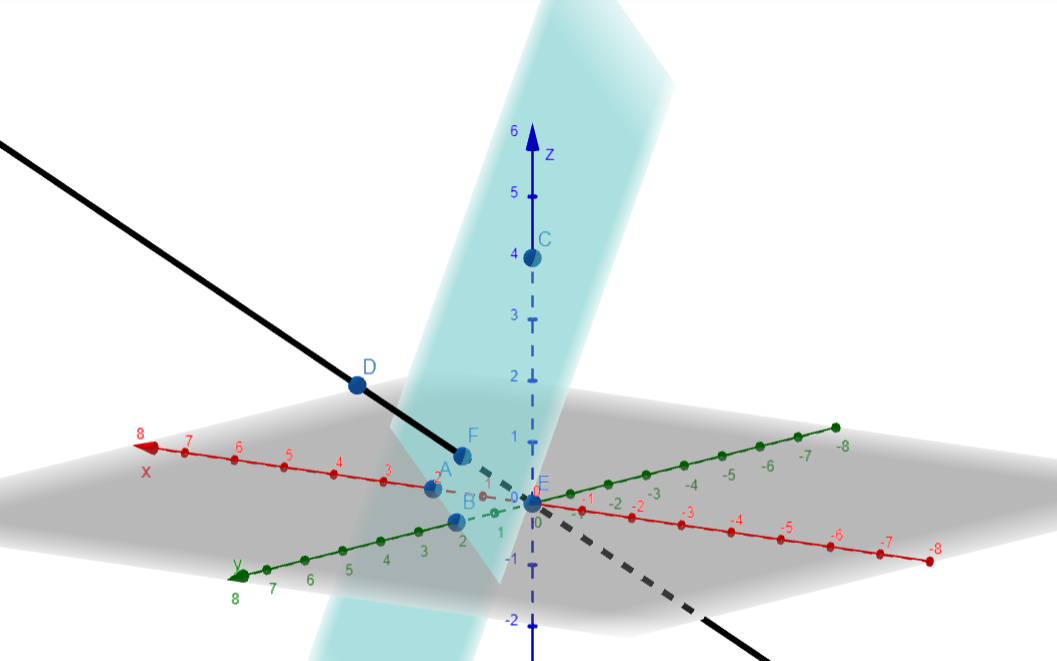
\includegraphics[width=0.7\textwidth]{GraficaEj2.png}
\caption{Grafica ejercicio 2}
\end{figure}

\subsection*{4. Comportamiento }
\begin{itemize}[leftmargin=1.5em]
\item Como $0 < s < 1$, el impacto ocurre antes de llegar al punto (2,2,2), es decir, la pared está entre el origen y ese punto.
\end{itemize}
\newpage
 

\section*{Ejercicio 3: Movimiento de un personaje (Recta en el espacio)}
\noindent\textbf{Puntos:} $A(2,1,0)$ y $B(5,7,3)$\\
 
\subsection*{1. Cálculo de la trayectoria}
\textbf{a) Vector director:}
\[
\vec{AB} = B - A = (5-2,\ 7-1,\ 3-0) = (3,6,3)
\]
\textbf{b) Ecuación vectorial del segmento:}
\[
\vec{r}(t) = A + t\,\vec{AB} = (2+3t,\ 1+6t,\ 3t), \qquad 0 \leq t \leq 1
\]
\begin{itemize}[leftmargin=1.5em]
\item Con t = 0 el personaje está en A y con t = 1 está en B, de modo que t representa la fracción del camino recorrido.
\item En el videojuego se incrementa t en cada cuadro hasta llegar a 1.
\item \textbf{Distancia total:} $\|\vec{AB}\| = \sqrt{3^2+6^2+3^2} = \sqrt{54} = 3\sqrt{6} \approx 7.35$ unidades.
\end{itemize}
\subsection*{2. Posición al 80\% del camino}
Se evalúa en $t = 0.8$:
\begin{align*}
x &= 2 + 3(0.8) = 4.4\\
y &= 1 + 6(0.8) = 5.8\\
z &= 0 + 3(0.8) = 2.4
\end{align*}
\textbf{Posición:} $(4.4,\ 5.8,\ 2.4)$
\subsection*{3. Comportamiento }
\begin{itemize}[leftmargin=1.5em]
\item El personaje se mueve en línea recta y a velocidad constante entre A y B.
\item Al 80\% del camino todavía le falta el 20\% de la distancia total, es decir, aproximadamente 1.47 unidades.
\end{itemize}
\newpage
 
%=====================================================================
\section*{Ejercicio 4: Operación Reconstrucción, sonda espacial corrupta (Superficies cuádricas)}
\noindent\textbf{Ecuaciones generales:}
\begin{itemize}[leftmargin=1.5em]
\item Módulo de energía (base): $x^2 + y^2 - z^2 + 2z - 2 = 0$
\item Cápsula de tripulación (centro): $4x^2 + 4y^2 + z^2 - 8z + 12 = 0$
\item Antena de comunicaciones (superior): $x^2 + y^2 - z + 6 = 0$
\item Núcleo de procesamiento (punta): $x^2 + y^2 + z^2 - 16z + 63.75 = 0$
\end{itemize}
 
\subsection*{1. Proceso algebraico (completar el cuadrado)}
Se usa la identidad $z^2 + bz = \left(z + \tfrac{b}{2}\right)^2 - \left(\tfrac{b}{2}\right)^2$.\\[0.3em]
\textbf{a) Módulo de energía (base):}
\begin{align*}
x^2 + y^2 - (z^2 - 2z) - 2 &= 0\\
x^2 + y^2 - \big[(z-1)^2 - 1\big] - 2 &= 0\\
x^2 + y^2 - (z-1)^2 &= 1
\end{align*}
Forma estándar: $\dfrac{x^2}{1} + \dfrac{y^2}{1} - \dfrac{(z-1)^2}{1} = 1$\\[0.5em]
\textbf{b) Cápsula de tripulación (centro):}
\begin{align*}
4x^2 + 4y^2 + \big[(z-4)^2 - 16\big] + 12 &= 0\\
4x^2 + 4y^2 + (z-4)^2 &= 4
\end{align*}
Forma estándar: $\dfrac{x^2}{1} + \dfrac{y^2}{1} + \dfrac{(z-4)^2}{4} = 1$\\[0.5em]
\textbf{c) Antena de comunicaciones (superior):}\\
Como z aparece solo a la primera potencia no se completa cuadrado, se despeja z:
\[
z - 6 = x^2 + y^2
\]
Forma estándar: $\dfrac{z-6}{1} = \dfrac{x^2}{1} + \dfrac{y^2}{1}$\\[0.5em]
\textbf{d) Núcleo de procesamiento (punta):}
\begin{align*}
x^2 + y^2 + \big[(z-8)^2 - 64\big] + 63.75 &= 0\\
x^2 + y^2 + (z-8)^2 &= 0.25
\end{align*}
Forma estándar: $\dfrac{x^2}{0.25} + \dfrac{y^2}{0.25} + \dfrac{(z-8)^2}{0.25} = 1$
\subsection*{2. Identificación de las superficies}
\begin{center}
\begin{tabular}{|c|c|c|c|}
\hline
\textbf{Pieza} & \textbf{Superficie} & \textbf{Centro / vértice} & \textbf{Datos} \\ \hline
Base & Hiperboloide de una hoja & (0, 0, 1) & a = b = c = 1 \\ \hline
Cápsula & Elipsoide & (0, 0, 4) & a = b = 1, c = 2 \\ \hline
Antena & Paraboloide & (0, 0, 6) & abre hacia $+z$ \\ \hline
Núcleo & Esfera & (0, 0, 8) & r = 0.5 \\ \hline
\end{tabular}
\end{center}
Los rangos de z del código base coinciden con estos resultados: la cápsula va de $4-2=2$ a $4+2=6$, la esfera de 7.5 a 8.5, y la antena inicia en su vértice z = 6.
\subsection*{3. Graficación en Mathematica}
\begin{figure}[H]
\centering
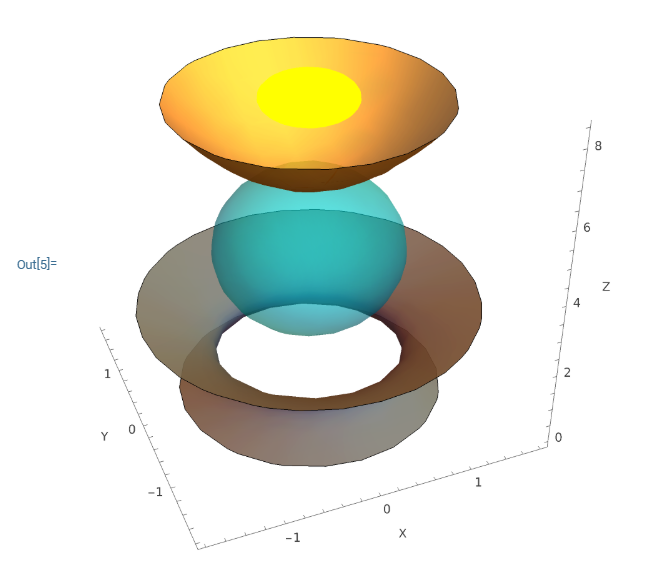
\includegraphics[width=0.45\textwidth]{Ej4Norm.png}\hfill
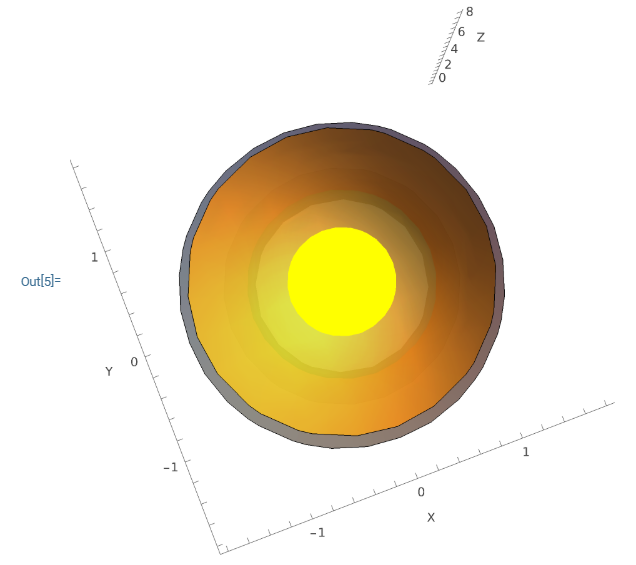
\includegraphics[width=0.45\textwidth]{Ej4Arrib.png}\\[0.5em]
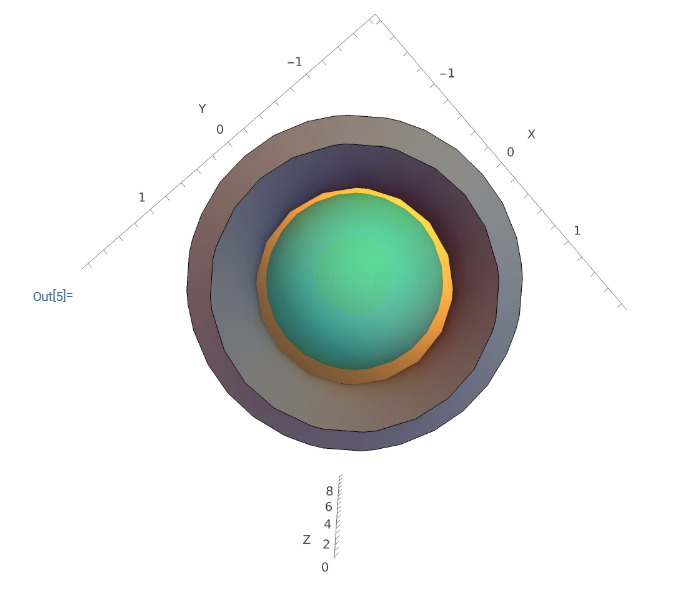
\includegraphics[width=0.45\textwidth]{Ej4Abaj.png}\hfill
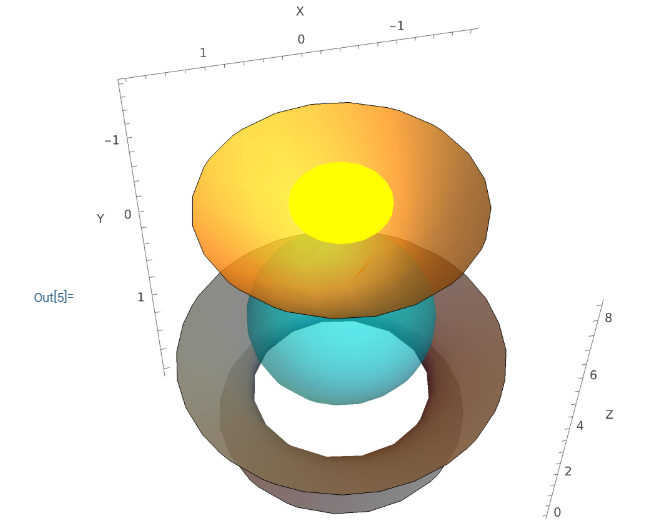
\includegraphics[width=0.45\textwidth]{Ej4DIAG.png}
\caption{Ejercicio 4: sonda espacial desde cuatro ángulos diferentes}
\end{figure}

\subsection*{5. Comportamiento }
\begin{itemize}[leftmargin=1.5em]
\item Las cuatro piezas comparten el mismo eje z, por eso se apilan una sobre otra y forman la sonda completa.
\item La base es opaca y oscura para que parezca metal, la cápsula es casi transparente como un cristal y el núcleo brilla con Glow para destacar en la punta.
\end{itemize}
\newpage
 
\end{document}
 